%---------------------------------------------------------------------------------------
%	META IMAGE
%----------------------------------------------------------------------------------------
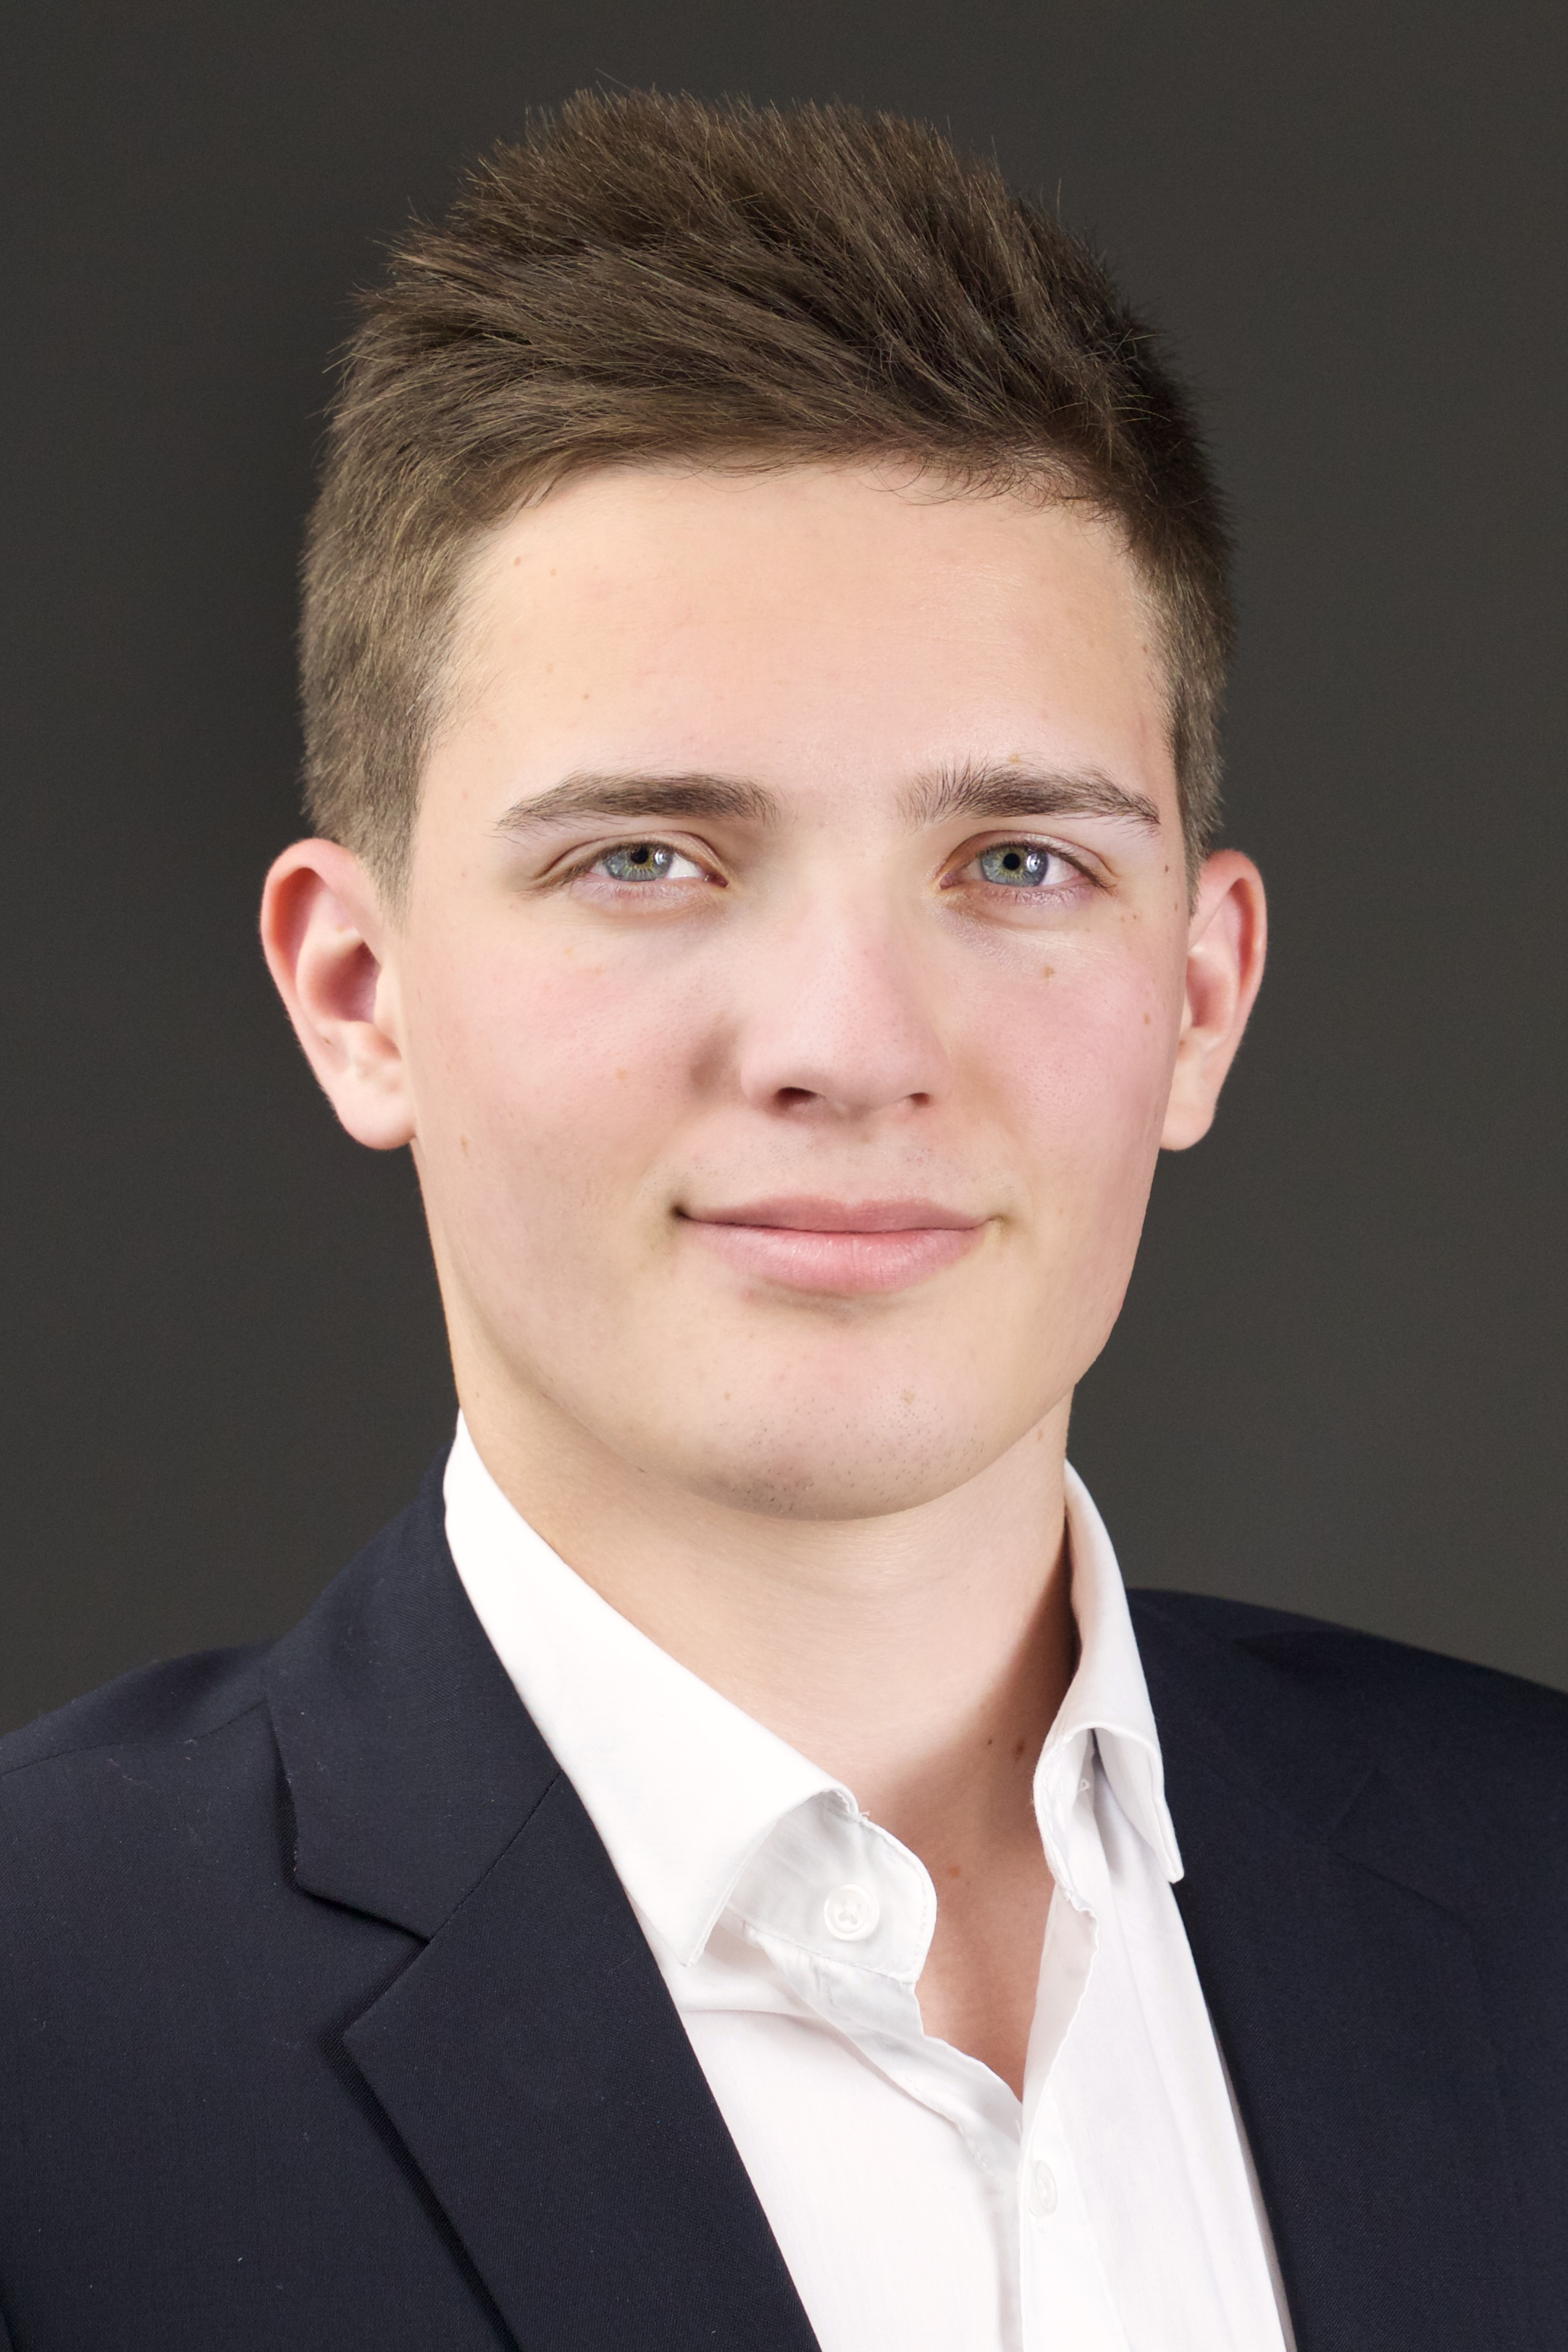
\includegraphics[width=\linewidth]{../resources/visage.jpg}	%trimming relative to image size

%---------------------------------------------------------------------------------------
%	META SKILLS
%----------------------------------------------------------------------------------------
\fcolorbox{white}{white}{\begin{minipage}[c][1.5cm][c]{1\mpwidth}
		\LARGE{\textbf{\textcolor{maincol}{Philip Empl}}} \\[2pt]
		\normalsize{ \textcolor{maincol} {Wirtschaftsinformatik (M. Sc.)} }
\end{minipage}} \\
\icontext{CaretRight}{12}{20.08.1995 in Trostberg}{black}\\[6pt]
\icontext{CaretRight}{12}{deutsch}{black}\\[6pt]
\icontext{CaretRight}{12}{ledig}{black}\\[6pt]



\cvsection{Fähigkeiten}

\cvskill{MATLAB \& Simulink} {5+ Jahre} {1} \\[-2pt]

\cvskill{Ansys Maxwell} {4+ Jahre} {0.667} \\[-2pt]

\cvskill{FEMM} {4+ Jahre} {0.667} \\[-2pt]

\cvskill{Webentwicklung} {2+ Jahre} {0.32} \\[-2pt]

\cvskill{Cloud Computing} {1+ Jahre} {0.16} \\[-2pt] \\

\cvskill{Deutsch} {L1} {1} \\[-2pt]

\cvskill{Englisch} {C1} {0.9} \\[-2pt]

\cvskill{Französisch} {B2} {0.4} \\[-2pt]

\newpage
%---------------------------------------------------------------------------------------
%	EDUCATION
%----------------------------------------------------------------------------------------
\cvsection{Bildung}

\cvmetaevent
{10/2017 - 07/2020}
{Wirtschaftsinformatik (M. Sc.)}
{Universität Regensburg}
{\textit{IT-Sicherheit • Data Science} \newline Masterarbeit: \glqq Vom Edge zur Cloud: eine explorative Studie zum Austausch und der Analyse von IoT-Daten\grqq.}
\cvmetaevent
{10/2014 - 08/2017}
{Wirtschaftsinformatik (B. Sc.)}
{Universität Regensburg}
{\textit{IT-Sicherheit • E-Commerce} \newline Bachelorarbeit: \glqq Addressing the inefficiency of searching backward: a novel tool to support authors of literature reviews\grqq.}

\cvmetaevent
{09/2006 - 06/2014}
{Allgemeines Abitur}
{Maximillian-von-Montgelas Gymnasium Vilsbiburg}
{\textit{Mathematik • Deutsch • Englisch • Wirtschaft • Musik}.}


%
%\cvsection{Projekte}

%	\cvlist{
	%		\item \hyperlink{https://github.com/philipempl/ether-twin}{\textbf{Ether-Twin.}}\\ Ethereum Applikation für Digital Twins.
	%		\item \hyperlink{https://github.com/philipempl/Peter-Pan}{\textbf{Peter Pan.}}\\ Koch-App (t.b.a.).
	%		\item \hyperlink{https://github.com/philipempl/Innovation-Tool}{\textbf{Innovation Tool.}}\\ Webcrawler für \hyperlink{https://ibi.de/}{Ibi}.
	%		\item \hyperlink{https://github.com/philipempl/cozone}{\textbf{COZONE.}} \\ Soziales Netzwerk (t.b.a.).
	%		\item \hyperlink{https://github.com/geritwagner/enlit}{\textbf{ENLIT.}}\\ Exploring new Literature (Bachelorarbeit).
	%		\item \textbf{Crowdfunding.} \\Modul mit \hyperlink{https://senacor.com/}{Senacor} für \hyperlink{https://www.paydirekt.de/}{paydirekt}.
	%		}

\cvsection{Interessen}

\icontext{CaretRight}{12}{Gitarrist bei Edit.Sprinter}{black}\\[6pt]
\icontext{CaretRight}{12}{DIY Heimprojekte}{black}\\[6pt]
\icontext{CaretRight}{12}{Krafttraining}{black}\\[6pt]
\icontext{CaretRight}{12}{Smart Home}{black}\\[6pt]
\icontext{CaretRight}{12}{Tierschutzverein Regensburg e.V.}{black}\\[6pt]




\cvsection{Kontakt}

\icontext{MapMarker}{16}{Kumpfmühler Str. 59\\93051 Regensburg}{black}\\[6pt]
\icontext{MobilePhone}{16}{+49 152 0986 5490}{black}\\[6pt]
\iconemail{Envelope}{16}{mail@philipempl.de}{mail@philipempl.de}{black}\\[6pt]
\iconhref{Home}{16}{htifs.uni-regensburg.de}{http://www.ifs.uni-regensburg.de}{black}\\[6pt]
\iconhref{Github}{16}{github.com/philipempl}{https://www.github.com/philipempl}{black}\\[6pt]
\iconhref{Xing}{16}{xing.com/Philip\_Empl}{https://www.xing.com/profile/Philip_Empl}{black}\\


%\cvqrcode{0.3}

